\documentclass{article}
\usepackage{amsmath}
\usepackage{amsfonts}
\usepackage{amssymb}
\usepackage{geometry}
\usepackage{graphicx}
\usepackage{placeins}
\usepackage{flafter}
\usepackage{xcolor}
\usepackage{listings}
\usepackage{algorithm}
\usepackage{algpseudocode}
\usepackage{hyperref}
\usepackage{enumitem}
\usepackage[affil-it]{authblk}
\geometry{a4paper, margin=1in}

\title{Algorithmic Methods for Mathematical Models\\
 Course Project}
\author{Marco Bartoli, Ilan Vezmarovic \\
    UPC Universitat Politècnica de Catalunya}

\begin{document}

\maketitle

\section{Formal Problem Definition}

\subsection{Inputs}

\begin{itemize}
    \item $n$: number of products
    \item $x$: height of the suitcase in millimeters
    \item $y$: width of the suitcase in millimeters
    \item $c$: limit to the total weight of the suitcase in grams
    \item $p_i$: price of the $i$-th product in euros
    \item $w_i$: weight of the $i$-th product in grams
    \item $s_i$: side length of the $i$-th product's (square) box in millimeters
\end{itemize}

\subsection{Outputs}

\begin{itemize}
    \item Indices of the products chosen to maximize the accumulated price
    \item Arrangement of the products in the suitcase
\end{itemize}

\section{Mathematical Formulation}

\subsection{Decision Variables}

\begin{itemize}
    \item $\text{Chosen}_i$: binary variable that is 1 if object $i$ is chosen, and 0 otherwise.
    \item $\text{PointsX}_i$: the x-coordinate of the bottom-left corner of object $i$.
    \item $\text{PointsY}_i$: the y-coordinate of the bottom-left corner of object $i$.
    \item $\text{Overlap}_{i,j,d}$: binary variable indicating if objects $i$ and $j$ do not overlap in direction $d$, where $d \in \{1, 2, 3, 4\}$.
\end{itemize}

\subsection{Objective Function}

Maximize the total price of the chosen objects:

\[
\text{maximize} \sum_{i=1}^n p_i \cdot \text{Chosen}_i
\]

\subsection{Constraints}

\subsubsection{Max Weight Constraint}

Ensure the total weight of the chosen objects does not exceed the suitcase's capacity:

\[
\sum_{i=1}^n w_i \cdot \text{Chosen}_i \leq c
\]

\subsubsection{Coordinate Bounds Constraints}

Ensure each object lies entirely within the suitcase's boundaries:

\[
\forall i \in \{1, \ldots, n\}, \quad \text{PointsX}_i \geq 1
\]

\[
\forall i \in \{1, \ldots, n\}, \quad \text{PointsY}_i \geq 1
\]

\[
\forall i \in \{1, \ldots, n\}, \quad \text{PointsX}_i + s_i - 1 \leq x
\]

\[
\forall i \in \{1, \ldots, n\}, \quad \text{PointsY}_i + s_i - 1 \leq y
\]

\subsubsection{Non-Overlapping Constraints}

Ensure no two chosen objects overlap within the suitcase using the big-M method:

1. Horizontal non-overlapping to the right:

\[
\forall i, j \in \{1, \ldots, n\}, i \neq j, \quad \text{PointsX}_i - \text{PointsX}_j + s_i \leq -M \cdot (\text{Chosen}_i + \text{Chosen}_j + \text{Overlap}_{i,j,1} - 3)
\]

2. Horizontal non-overlapping to the left:

\[
\forall i, j \in \{1, \ldots, n\}, i \neq j, \quad \text{PointsX}_j - \text{PointsX}_i + s_j \leq -M \cdot (\text{Chosen}_i + \text{Chosen}_j + \text{Overlap}_{i,j,2} - 3)
\]

3. Vertical non-overlapping upwards:

\[
\forall i, j \in \{1, \ldots, n\}, i \neq j, \quad \text{PointsY}_i - \text{PointsY}_j + s_i \leq -M \cdot (\text{Chosen}_i + \text{Chosen}_j + \text{Overlap}_{i,j,3} - 3)
\]

4. Vertical non-overlapping downwards:

\[
\forall i, j \in \{1, \ldots, n\}, i \neq j, \quad \text{PointsY}_j - \text{PointsY}_i + s_j \leq -M \cdot (\text{Chosen}_i + \text{Chosen}_j + \text{Overlap}_{i,j,4} - 3)
\]

\subsubsection{At Least One Not Overlapping Constraint}

Ensure that for any two objects, at least one of the non-overlapping conditions is satisfied:

\[
\forall i, j \in \{1, \ldots, n\}, i \neq j, \quad \sum_{d=1}^4 \text{Overlap}_{i,j,d} \geq 1
\]

\newpage

\section{Heuristic}

\subsection{Greedy Algorithm}
A greedy algorithm makes the optimal choice at each step by selecting products based on $Qvalue = \frac{price}{side \times weight}$.

\subsubsection{Pseudocode}
\begin{algorithm}
\caption{Greedy Algorithm}
\begin{algorithmic}
    \State \textbf{Input:} A problem instance with $n$ products, suitcase dimensions $(x, y)$, and weight capacity $c$.
    \State \textbf{Output:} A feasible solution with selected products that maximize the total price.    

    \State Initialize solution as empty
    \State Sort products by $(price / side / weight)$ in descending order

    \For{each product in sorted products}
        \If{product can fit in the suitcase and does not exceed weight limit}
            \State Add product to solution
            \State Update suitcase dimensions and weight capacity
        \EndIf
    \EndFor

    \State \Return solution
\end{algorithmic}
\end{algorithm}

\section{Meta-heuristics}

\subsection{Local Search Algorithm}
After constructing an initial solution using the greedy algorithm, a local search is applied to improve it by exploring neighboring solutions.

\subsubsection{Pseudocode}
\begin{algorithm}
\caption{Local Search Algorithm}
\begin{algorithmic}
    \State \textbf{Input:} An initial solution, mode (FIRST\_IMPROVEMENT or BEST\_IMPROVEMENT), strategy (EXCHANGE or REASSIGNMENT)
    \State \textbf{Output:} An improved solution

    \State bestSolution = initialSolution
    \State improved = true
        
    \While{improved}
        \State improved = false

        \For{each product in bestSolution}
            \If{strategy == EXCHANGE}
                \State newSolution = exchangeProduct(bestSolution, product)
            \ElsIf{strategy == REASSIGNMENT}
                \State newSolution = reassignProduct(bestSolution, product)
            \EndIf

            \If{newSolution is better than bestSolution}
                \State bestSolution = newSolution
                \State improved = true
                
                \If{mode == FIRST\_IMPROVEMENT}
                    \State \Return bestSolution
                \EndIf
            \EndIf
        \EndFor
    \EndWhile

    \State \Return bestSolution
\end{algorithmic}
\end{algorithm}

\begin{algorithm}
\caption{Exchange Product}
\begin{algorithmic}
    \State \textbf{Input:} A solution, a product to be exchanged
    \State \textbf{Output:} A new solution with the product exchanged

    \State bestSolution = initialSolution
    \State newProductList = copy of the selected product list from the solution
    \State remove the selected product from newProductList

    \For{each unselected product}
        \State add unselected product to newProductList
        \State newSolution = findSolutionForProductList(newProductList)
        
        \If{newSolution is better than bestSolution}
            \State bestSolution = newSolution

            \If{mode == \texttt{FIRST\_IMPROVEMENT}}
                \State \Return bestSolution
            \EndIf
        \EndIf
        \State remove unselected product from newProductList        
    \EndFor

    \State \Return bestSolution
\end{algorithmic}
\end{algorithm}

\begin{algorithm}
\caption{Reassign Product}
\begin{algorithmic}
    \State \textbf{Input:} A solution, a product to be excluded for re-evaluation
    \State \textbf{Output:} A new solution with products reassigned

    \State bestSolution = initialSolution
    
    \For{each selected product}
        \State newProductList = copy of the all product list
        \State remove the selected product from newProductList
        
        \State newSolution = findSolutionForProductList(newProductList)    

        \If{newSolution is better than current solution}
            \State bestSolution = newSolution
    
            \If{mode == FIRST\_IMPROVEMENT}
                \State \Return bestSolution
            \EndIf
        \EndIf                
    \EndFor
    
    \State \Return bestSolution
\end{algorithmic}
\end{algorithm}


\subsection{GRASP (Greedy Randomized Adaptive Search Procedure)}
GRASP consists of a construction phase where a feasible solution is generated using a randomized greedy algorithm, followed by a local search to iteratively improve the solution. By default, GRASP uses \texttt{FIRST\_IMPROVEMENT} and \texttt{EXCHANGE} for local search.

\subsubsection{Pseudocode}
\begin{algorithm}
\caption{GRASP Algorithm}
\begin{algorithmic}
    \State \textbf{Input:} A problem instance, maxIterations, alpha (for RCL threshold)
    \State \textbf{Output:} The best solution found

    \State bestSolution = null

    \For{iteration = 1 to maxIterations}
        \State greedySolution = constructGreedyRandomizedSolution(problem, alpha)
        \State localOptimalSolution = LOCAL\_SEARCH(greedySolution, FIRST\_IMPROVEMENT)

        \If{bestSolution is null or localOptimalSolution is better than bestSolution}
            \State bestSolution = localOptimalSolution
        \EndIf
    \EndFor

    \State \Return bestSolution
\end{algorithmic}
\end{algorithm}

\begin{algorithm}
\caption{Construct Greedy Randomized Solution}
\begin{algorithmic}
    \State \textbf{Input:} A problem instance, alpha (for RCL threshold)
    \State \textbf{Output:} A feasible solution

    \State Initialize solution as empty
    \State Sort products by $(price / side / weight)$ in descending order

    \While{there are remaining products}
        \State $qMax$ = maximum $Q$ value in remaining products
        \State $qMin$ = minimum $Q$ value in remaining products
        \State threshold = $qMax - alpha \times (qMax - qMin)$

        \State RCL = \{products with $Q$ value $>=$ threshold\}
        \State selectedProduct = randomly select a product from RCL

        \If{selectedProduct fits in the suitcase and does not exceed weight limit}
            \State Add selectedProduct to solution
            \State Update suitcase dimensions and weight capacity
        \EndIf
    \EndWhile

    \State \Return solution
\end{algorithmic}
\end{algorithm}


\newpage

\section{Tuning Local Search}

\begin{figure}[!h]
    \centering
    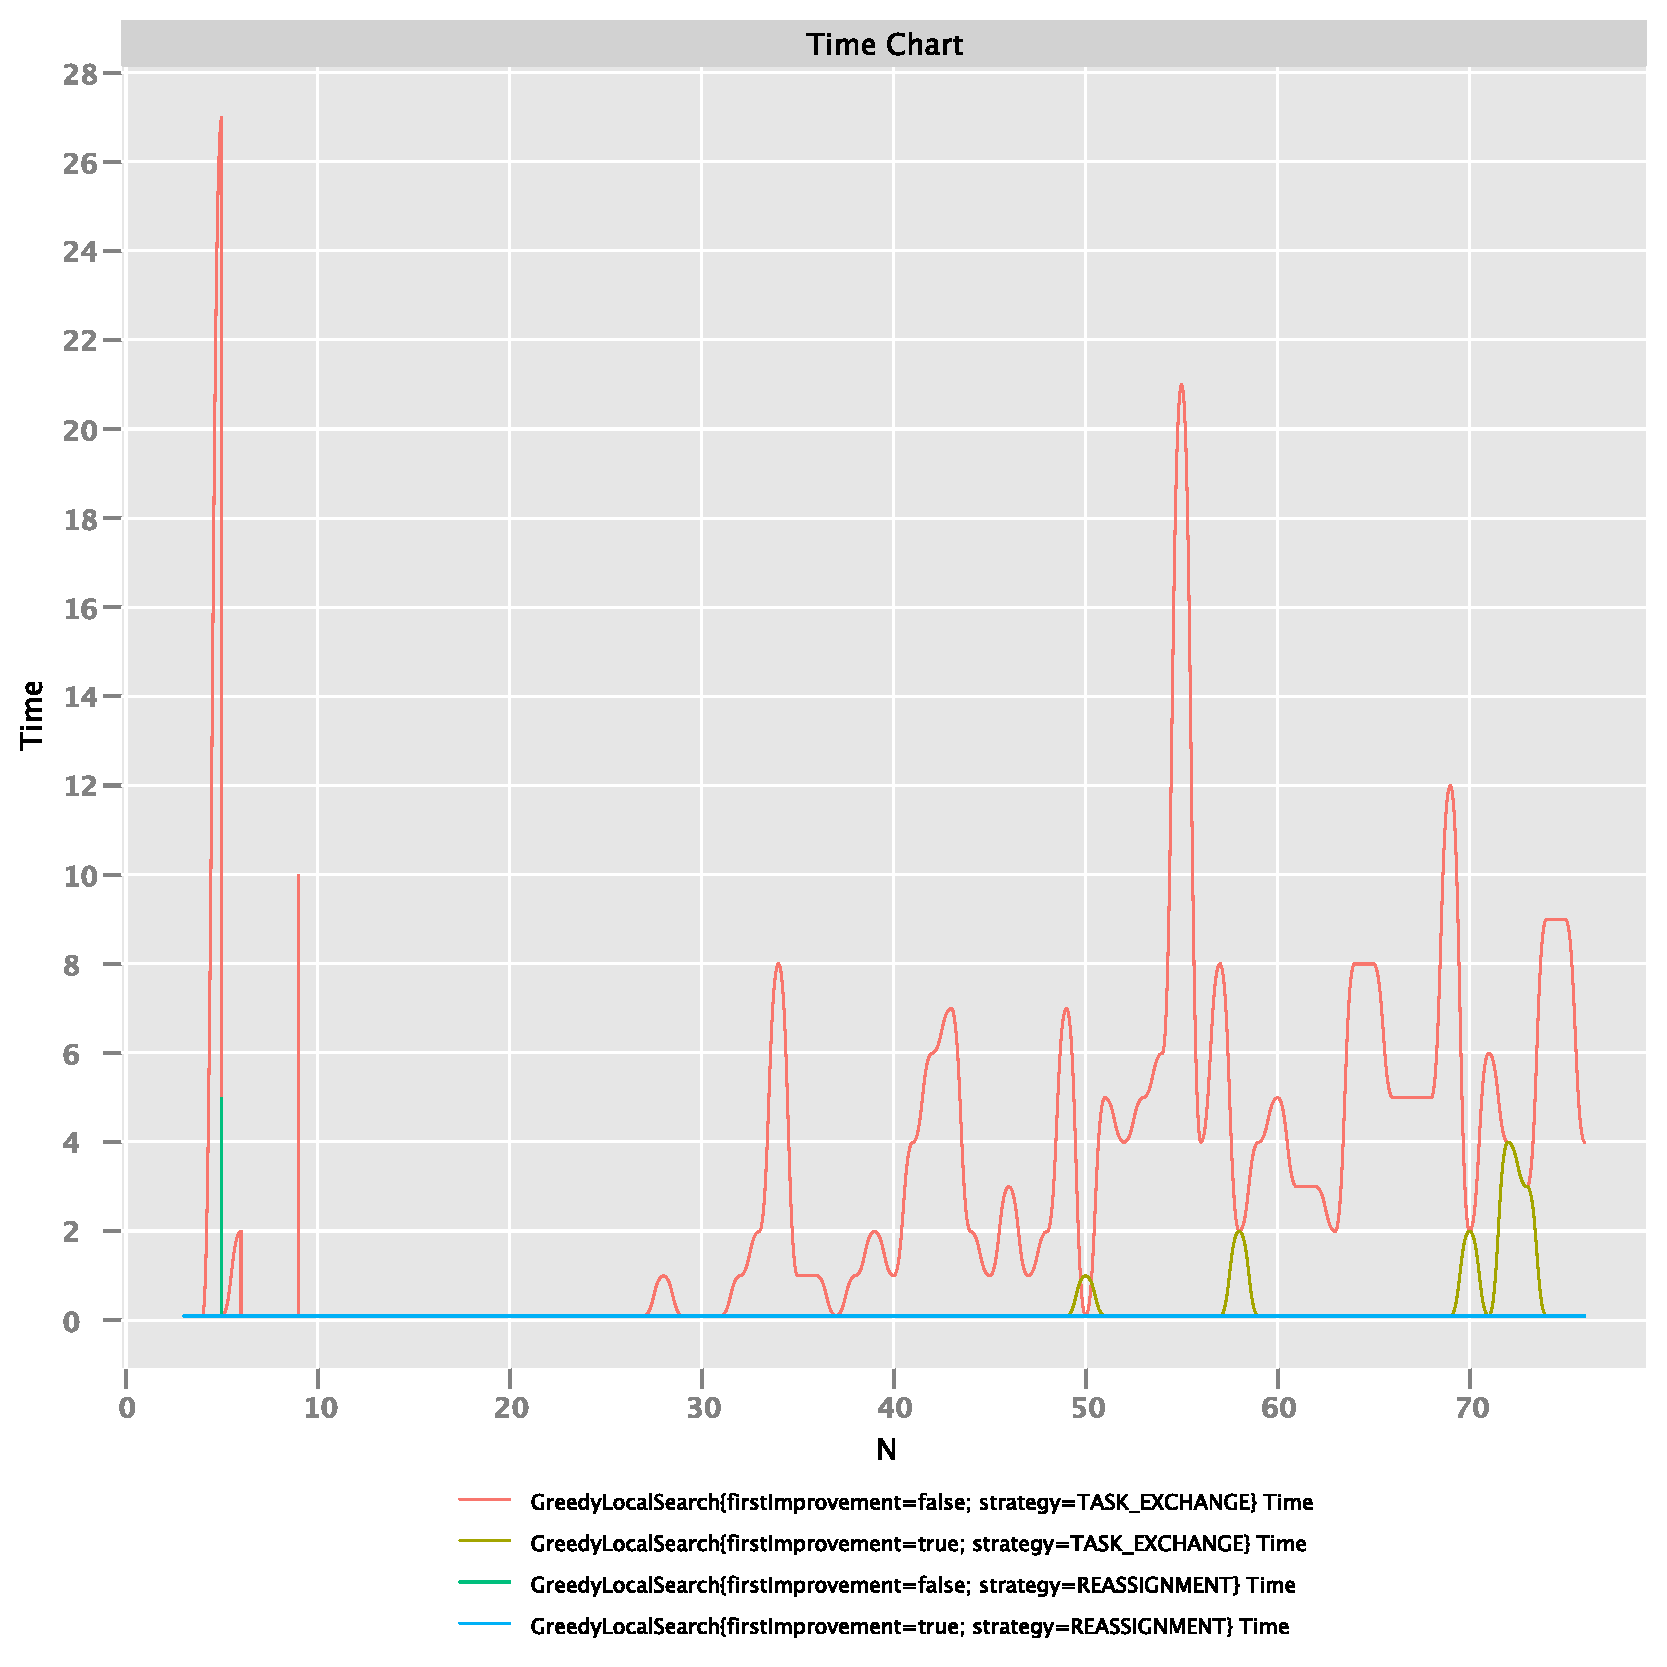
\includegraphics[width=0.9\textwidth]{./documentation/assets/new.localSearchParams.timeChart.pdf}
    \caption{Time Parameters Local Search}
    \label{fig:local_time}
\end{figure}\FloatBarrier

The results show a clear trade-off between execution time and solution quality. The Best Improvement strategy, especially with Task Exchange, produced the highest objective values but took much longer to run. On the other hand, Task Reassignment methods were the fastest but resulted in slightly lower objective values.

The First Improvement strategy, while faster, often settled for less optimal solutions compared to the Best Improvement strategy because it stops early upon finding the first better neighbor.

\begin{figure}[!h]
    \centering
    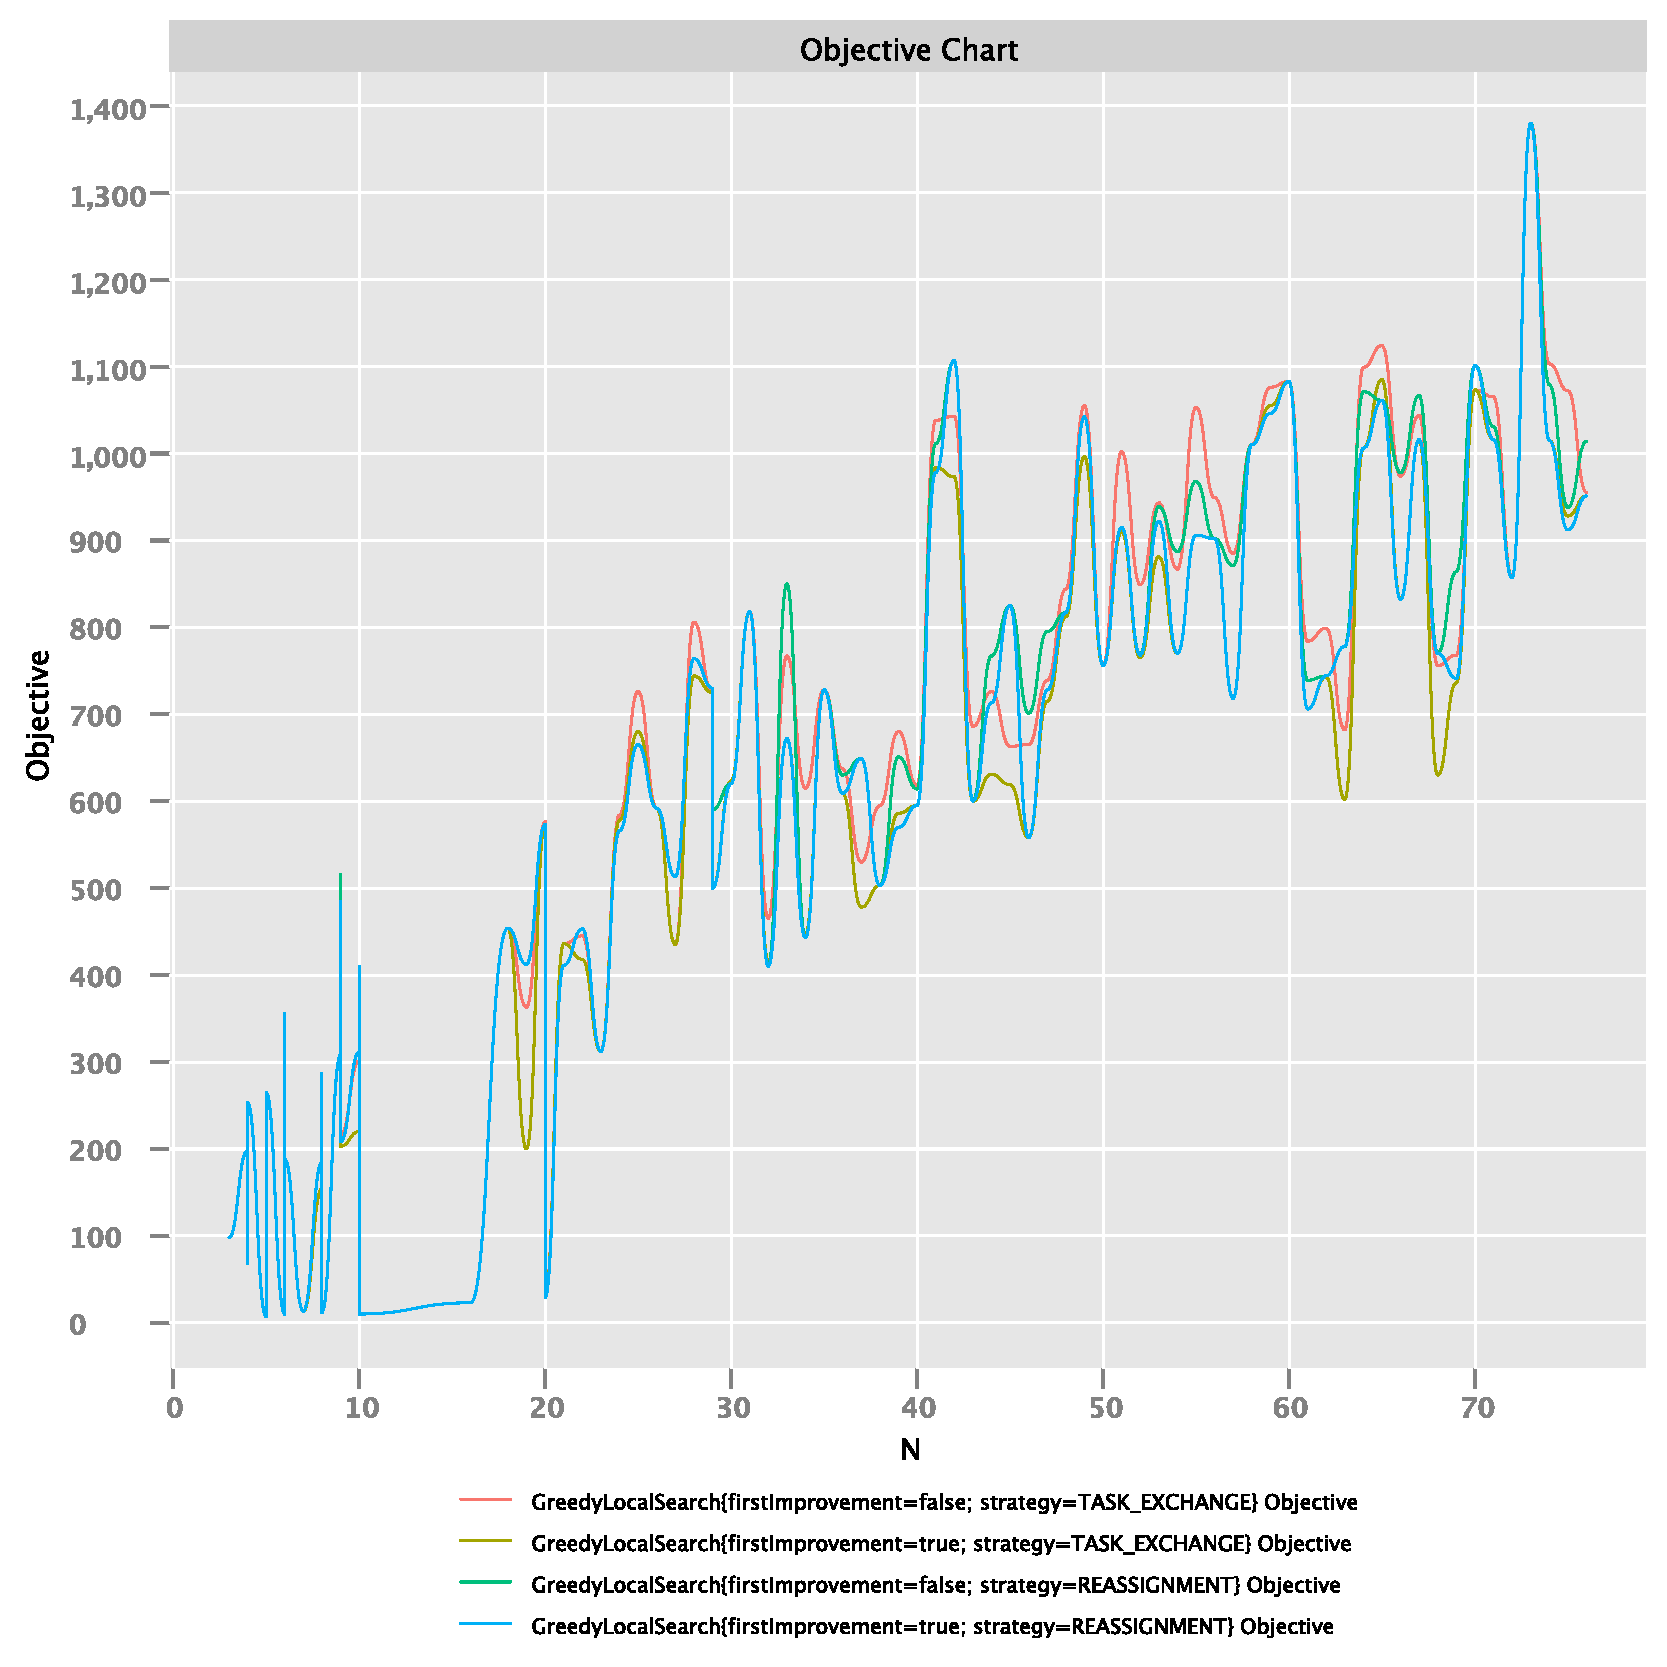
\includegraphics[width=1\textwidth]{./documentation/assets/new.localSearchParams.objectiveChart.pdf}
    \caption{Objective Parameters Local Search}
    \label{fig:local_objective}
\end{figure}\FloatBarrier

From the experiments, we can draw the following conclusions:
\begin{itemize}
    \item \textbf{Best Improvement + Task Exchange}: Best for scenarios where solution quality is most important, and higher execution times are acceptable.
    \item \textbf{First Improvement + Task Reassignment}: Best for scenarios requiring quick solutions with reasonably good quality.
    \item \textbf{Best Improvement + Task Reassignment}: Offers a balanced trade-off, providing good quality solutions within an acceptable time frame.
    \item \textbf{First Improvement + Task Exchange}: Not recommended due to less optimal solutions and slower performance compared to task reassignment.
\end{itemize}

\section*{Conclusion}
The Best Improvement strategy with Task Exchange is best for scenarios focusing on solution quality, despite longer execution times. On the other hand, the First Improvement strategy with Task Reassignment is preferable for scenarios needing quick solutions, balancing speed and solution quality well. The Best Improvement strategy with Task Reassignment offers a middle ground, providing good solutions within reasonable times. Therefore, the choice of strategy should match the specific needs for execution time and solution quality of the application. In this study, First Improvement and Reassignment were chosen to minimize time loss while maintaining satisfactory solution quality.


\newpage

\section{GRASP Parameter Tuning}

\begin{figure}[!h]
    \centering
    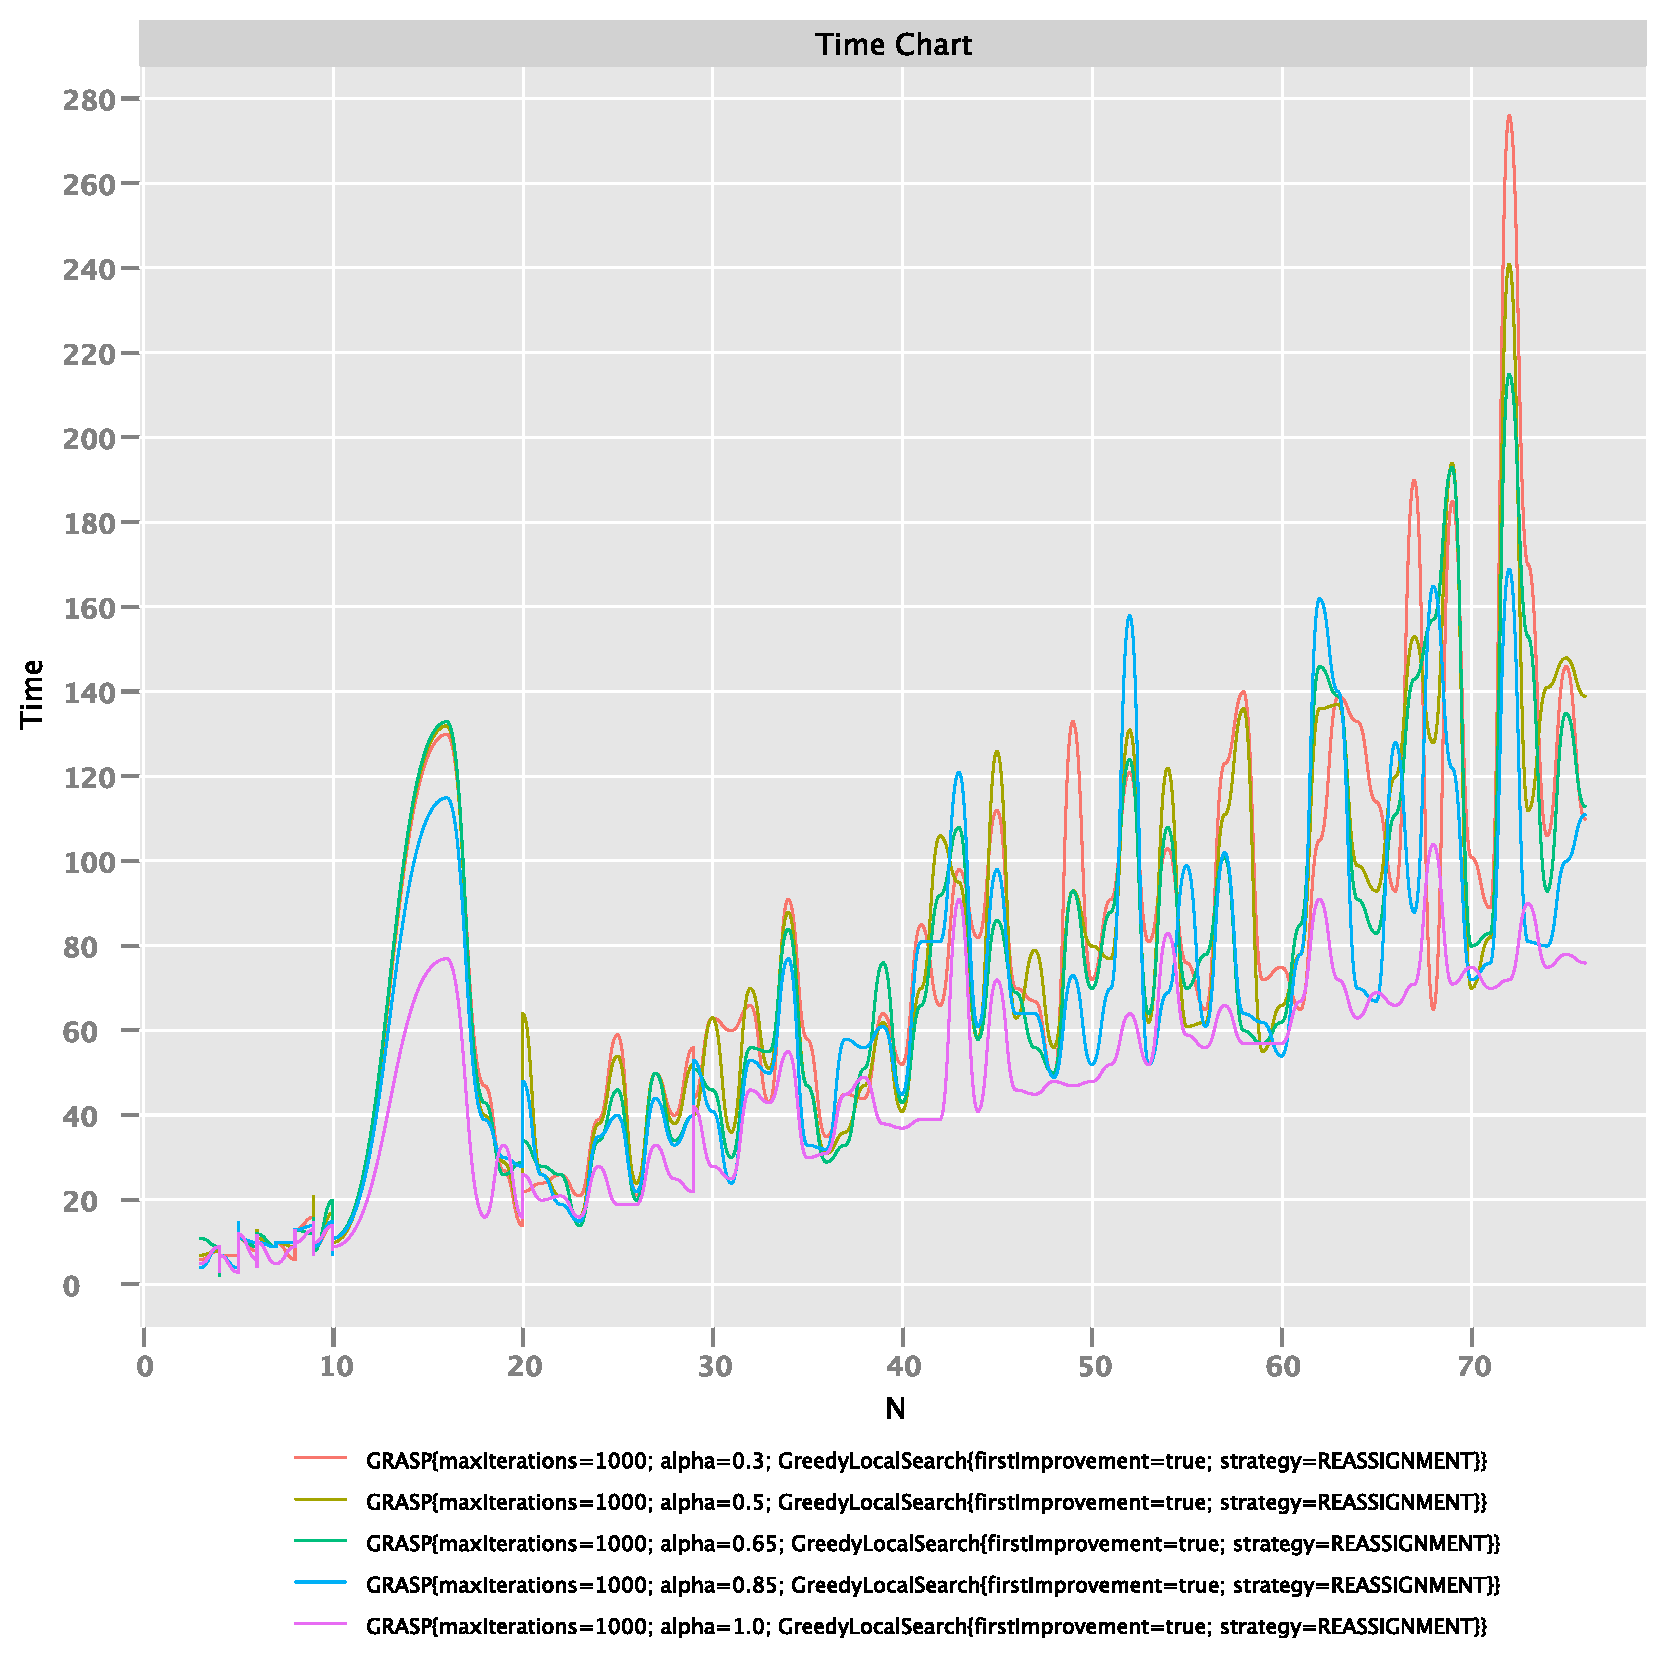
\includegraphics[width=0.9\textwidth]{./documentation/assets/new.GRASPParams.timeChart.pdf}
    \caption{Execution Time for Different Alpha Values in GRASP}
    \label{fig:grasp_time}
\end{figure}\FloatBarrier

The results indicate that the execution time for the GRASP algorithm is generally faster with higher alpha values. Specifically, alpha values closer to 1 (corresponding to purely random selection) resulted in the fastest execution times, while lower alpha values, like 0.3, resulted in slower execution times.

\begin{figure}[!h]
    \centering
    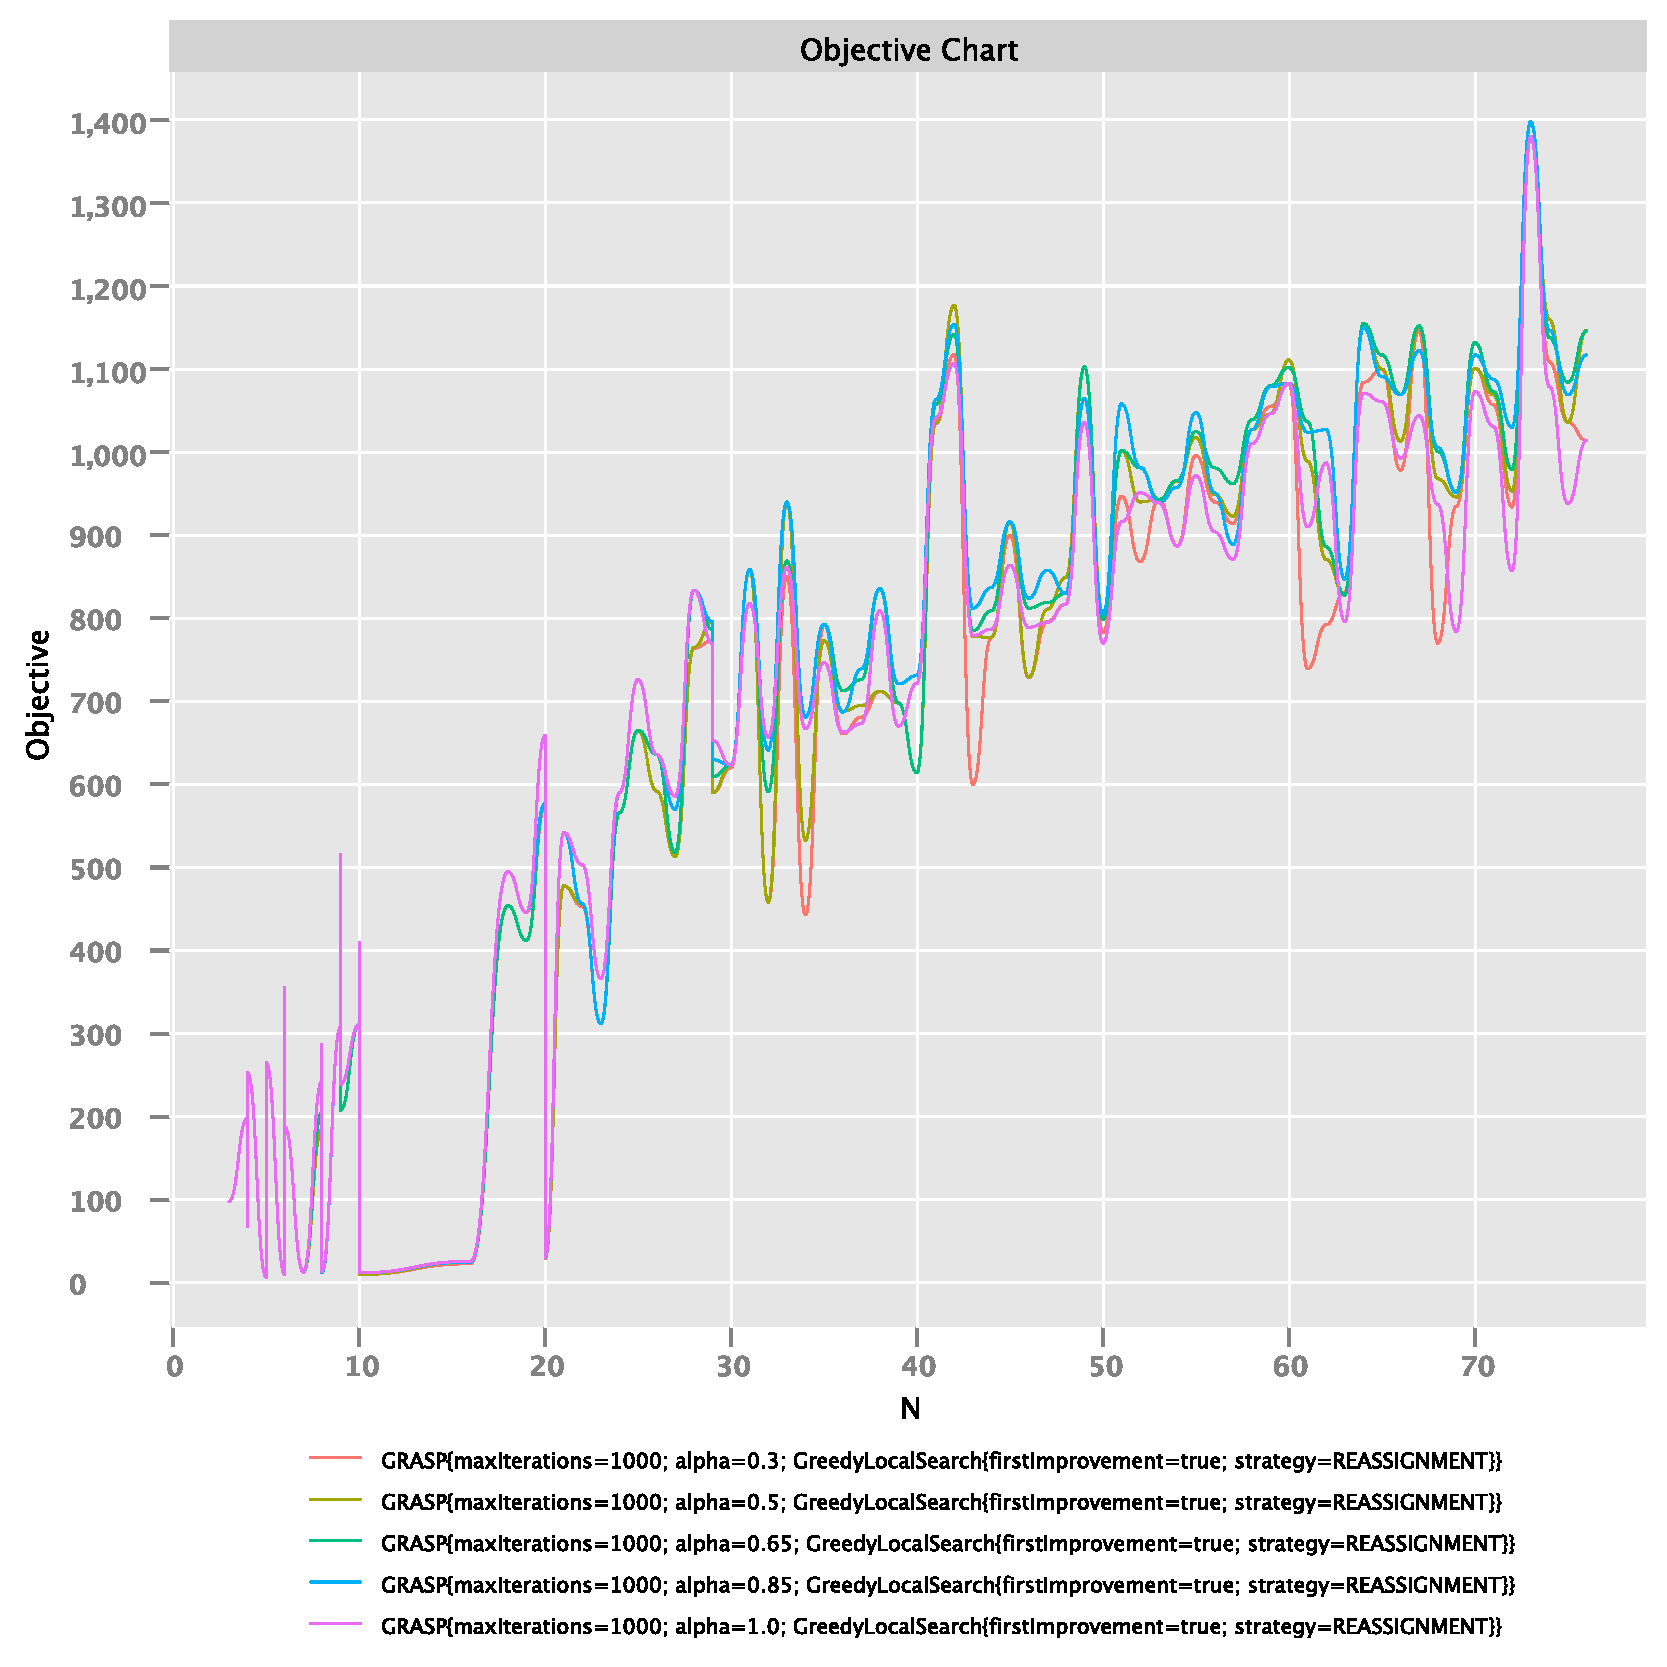
\includegraphics[width=1\textwidth]{./documentation/assets/new.GRASPParams.objectiveChart.pdf}
    \caption{Objective Values for Different Alpha Values in GRASP}
    \label{fig:grasp_objective}
\end{figure}\FloatBarrier

In terms of objective values, both the lowest (alpha = 0.3) and the highest (alpha = 1) alpha values produced the lowest objective values. The intermediate alpha values, particularly alpha = 0.65, resulted in the best objective values, suggesting a balanced approach between greedy and random selection generates better results.

\section*{Conclusion}
The experiments reveal that using a higher alpha value in the GRASP algorithm speeds up the execution time, but both very low and very high alpha values result in lower objective values. The best solution quality was obtained with an alpha value of 0.65, which strikes a balance between greedy and random selection. For practical applications, an alpha value around 0.65 is recommended to achieve a good balance between execution time and solution quality.

\newpage

\section{Overall Performance Graphs}

\begin{figure}[!h]
    \centering
    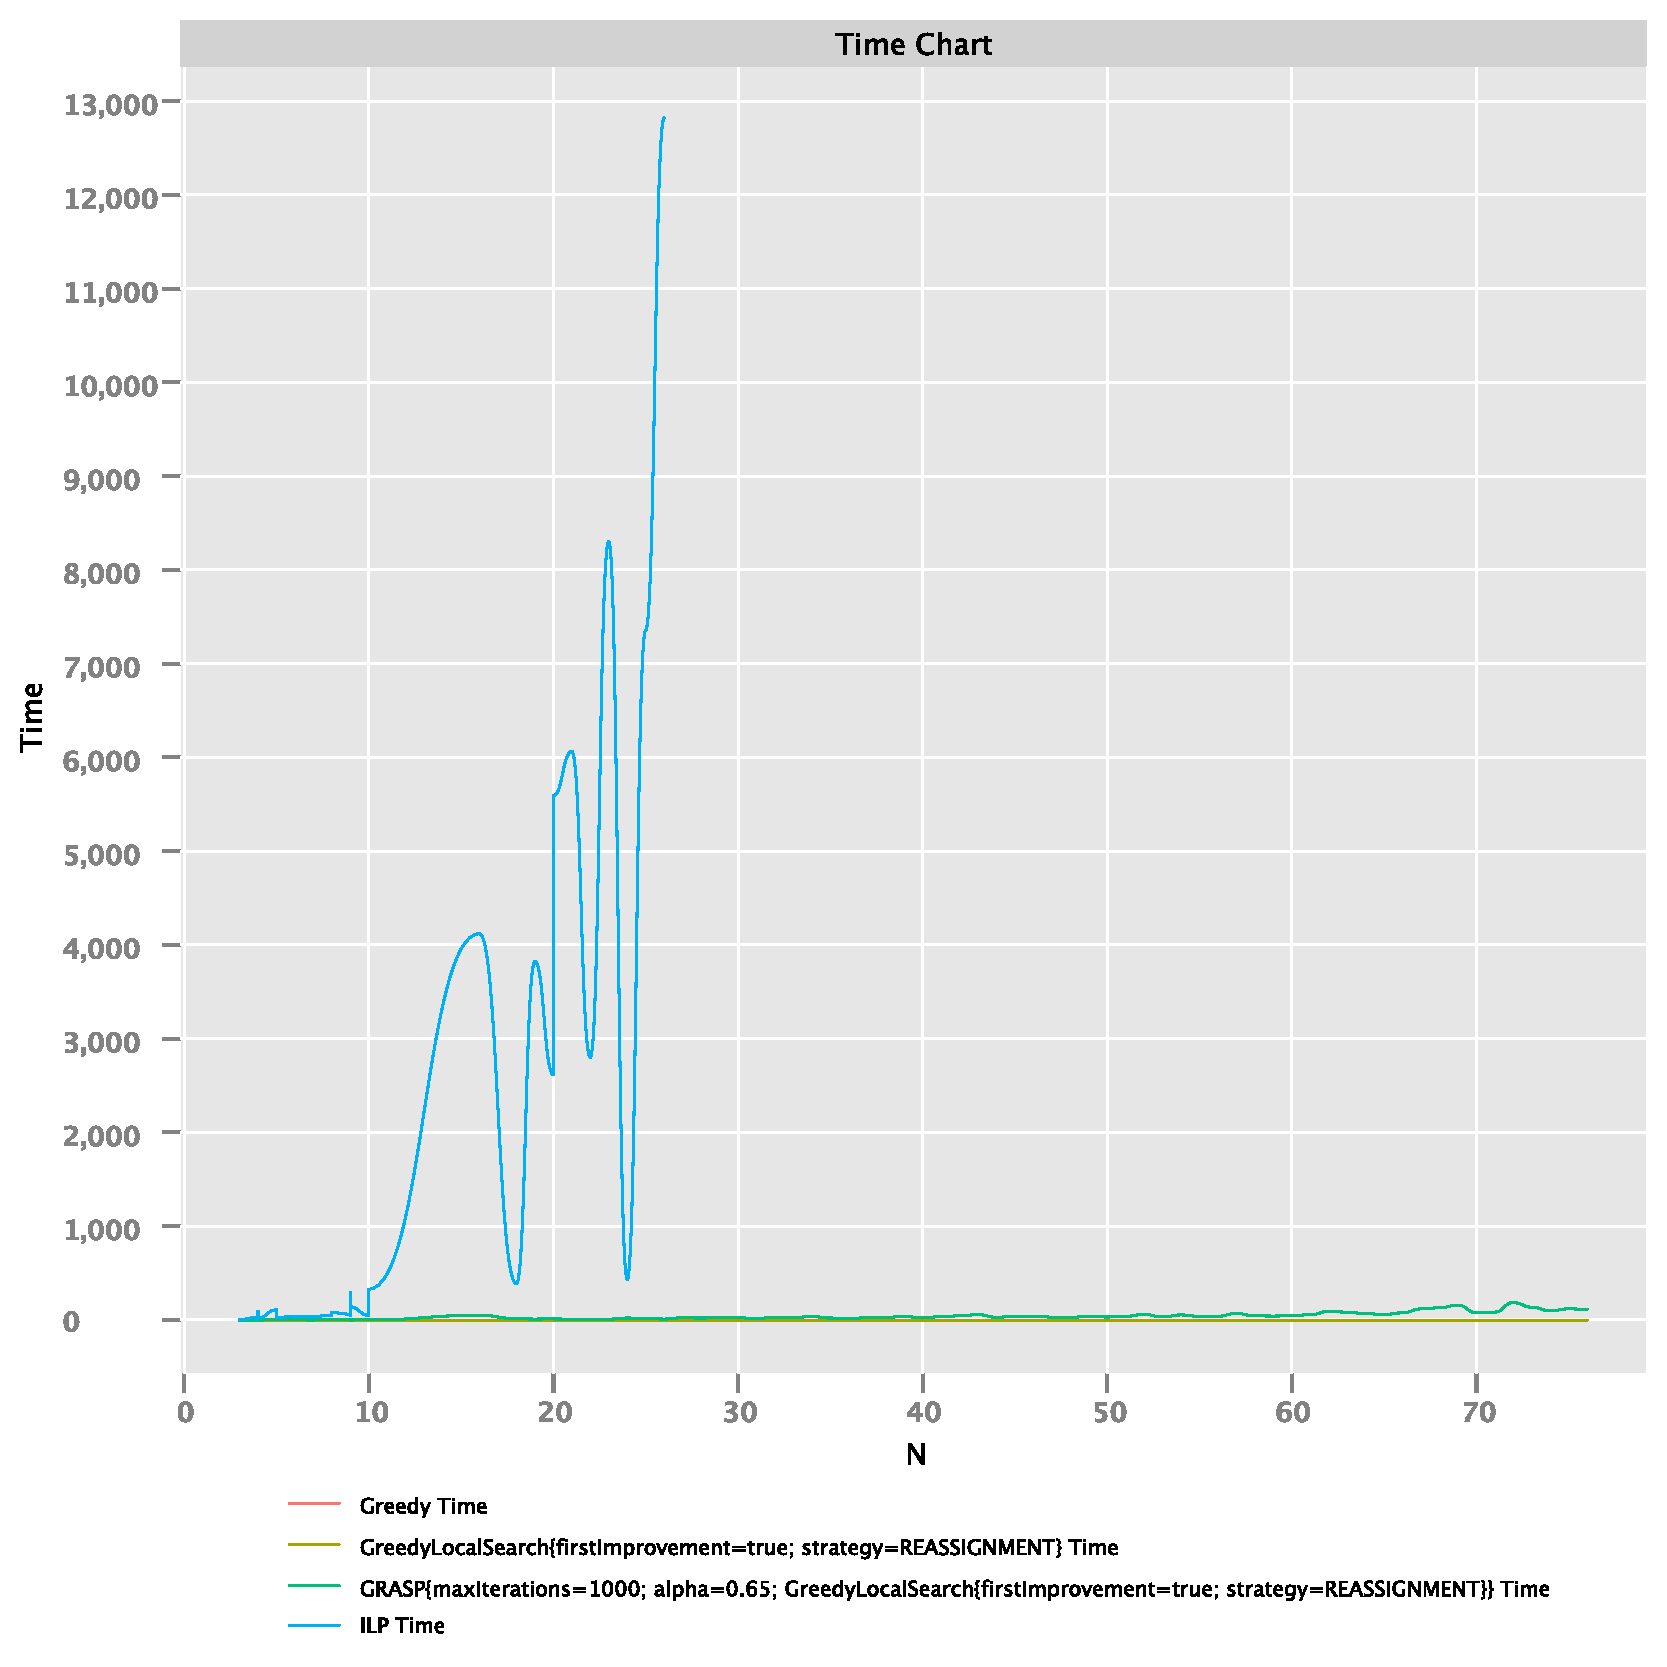
\includegraphics[width=1\textwidth]{./documentation/assets/new.all.timeChart.pdf}
    \caption{Execution Time for All Algorithms}
    \label{fig:all_time}
\end{figure}\FloatBarrier

\begin{figure}[!h]
    \centering
    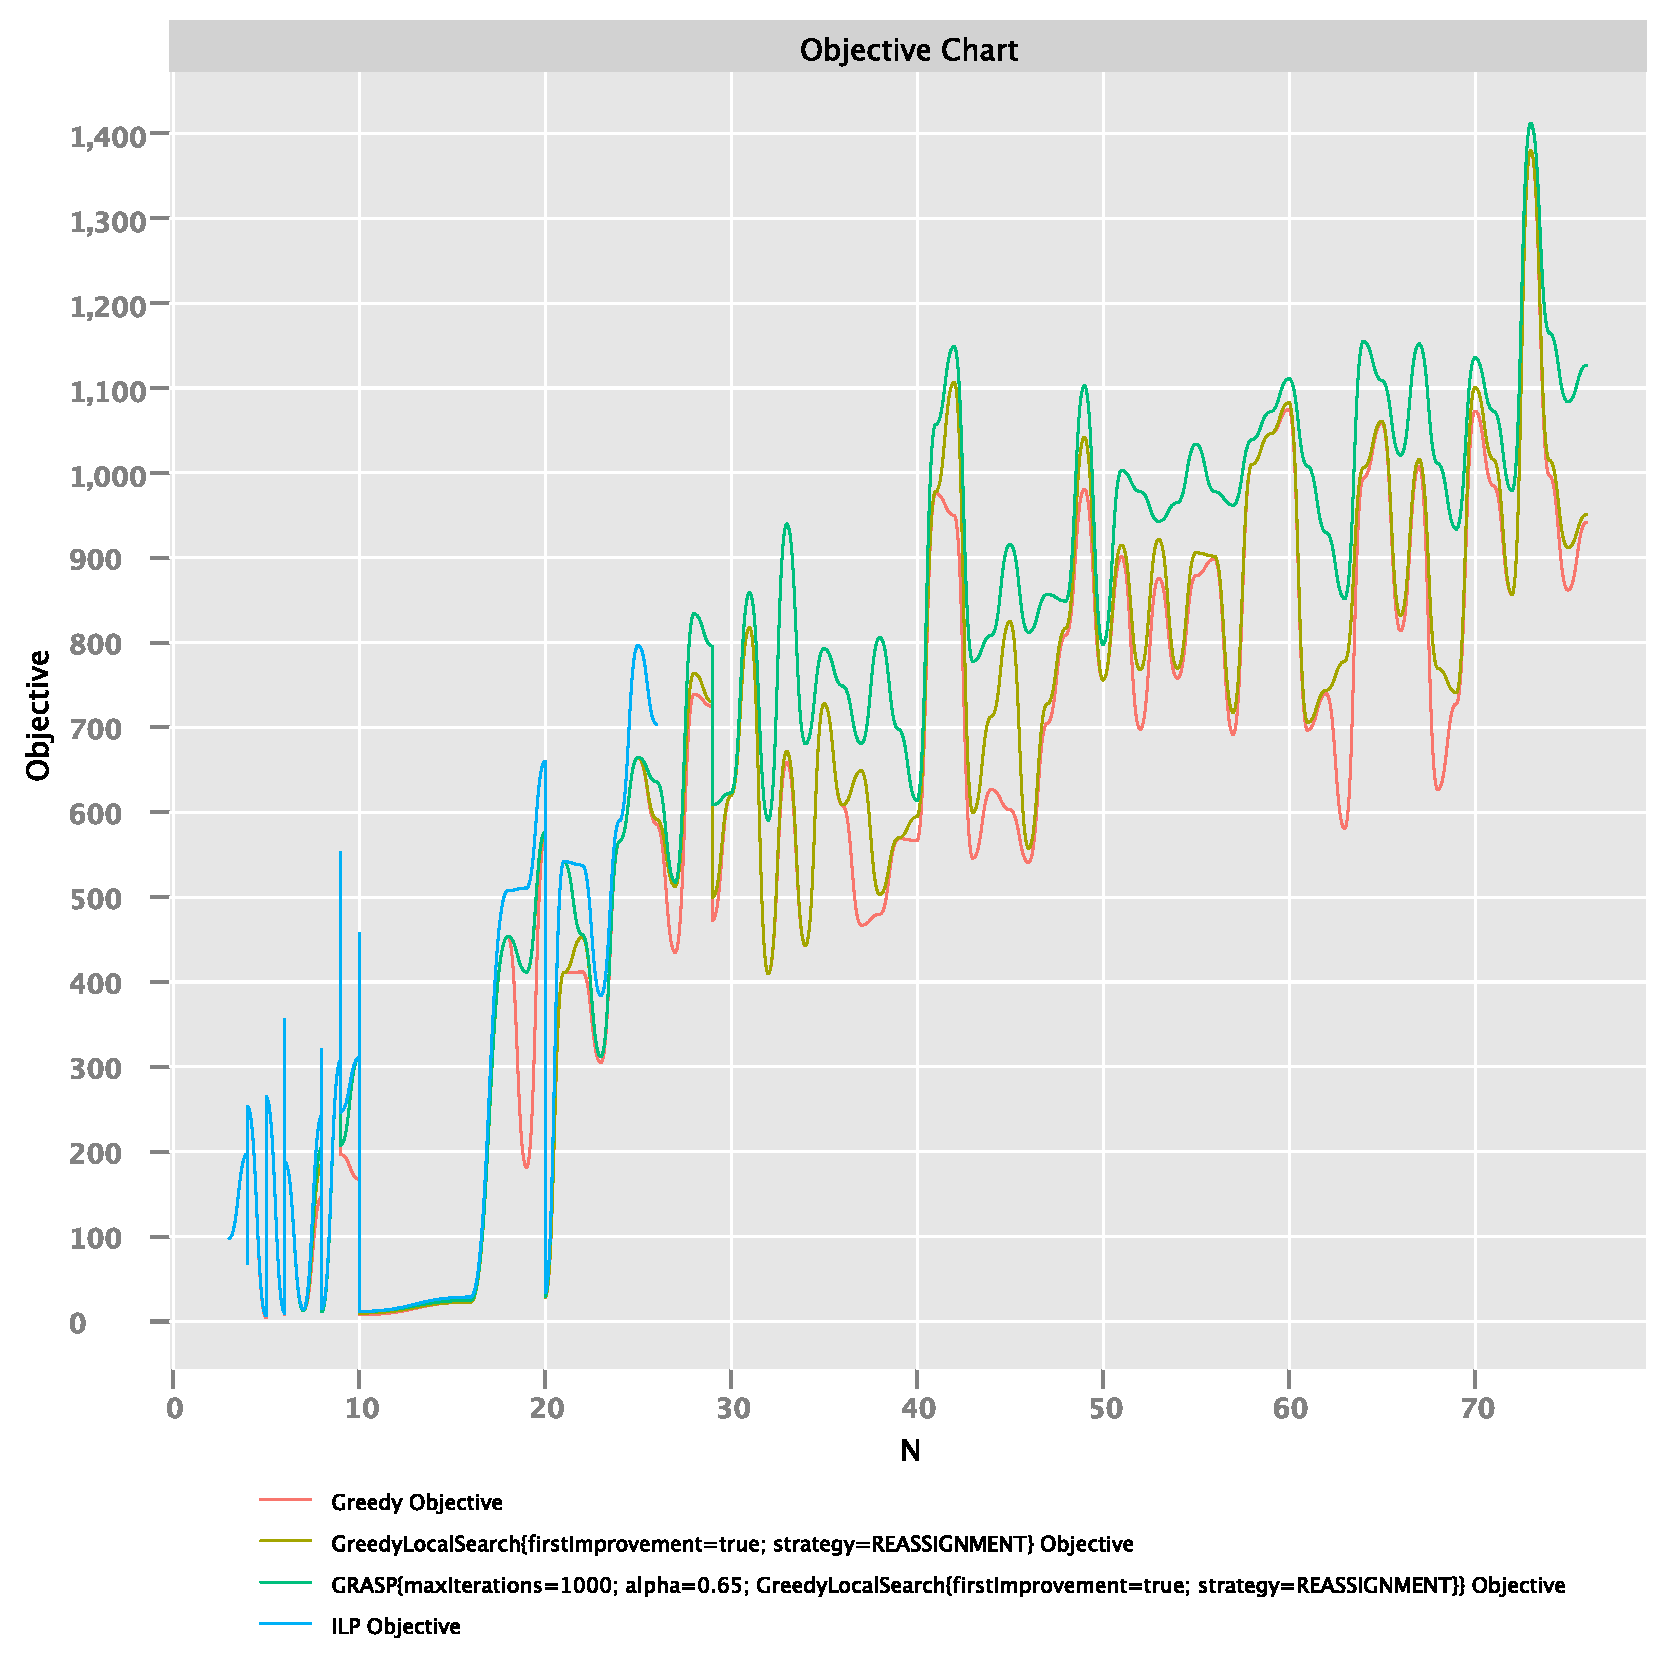
\includegraphics[width=1\textwidth]{./documentation/assets/new.all.objectiveChart.pdf}
    \caption{Objective Values for All Algorithms}
    \label{fig:all_objective}
\end{figure}\FloatBarrier

\newpage

\section{Conclusion}

The overall performance analysis reveals significant differences among the algorithms in both execution time and solution quality. The ILP algorithm consistently performed the worst, failing to provide a solution for instances where \( N > 27 \) within a 30-minute timeframe. This limitation makes ILP unsuitable for larger problem sizes.

In contrast, the Greedy algorithm provided quick solutions but often at the expense of solution quality. The addition of Local Search to the Greedy algorithm improved the solution quality considerably, particularly with the Best Improvement strategy combined with Task Exchange, although it required more time to execute.

The GRASP algorithm, with its different alpha parameters, demonstrated a good balance between execution time and solution quality. While higher alpha values (purely random selection) resulted in faster execution times, an intermediate alpha value, particularly around 0.65, yielded the best objective values. This suggests that a balanced approach between greedy and random selection is most effective.

In summary, for small to medium-sized problems where execution time is critical, the Greedy algorithm with Task Reassignment is preferable. For scenarios requiring high-quality solutions, the Best Improvement strategy with Task Exchange or GRASP with an alpha value of 0.65 offers the best results. ILP is impractical for larger instances due to its prohibitive execution times.


\section{How to run}

\begin{itemize}
  \item Install IBM CPLEX
  \item Install Java 22
  \item Install Maven
\end{itemize}

Those are the commands to run it from command line without using an IDE

This will run both OPL and Heuristic and output benchmark values in CSV.

\begin{lstlisting}[language=bash]
cd heuristic
mvn compile exec:java -Dexec.mainClass="edu.upc.fib.ammm.Main" -Dexec.args="../opl"
\end{lstlisting}

Make plots of a run

\begin{lstlisting}[language=bash]
mvn compile exec:java -Dexec.mainClass="edu.upc.fib.ammm.Plot" -Dexec.args="output.csv"
\end{lstlisting}

\end{document}